\documentclass[12pt,a4paper,oneside]{report}
\usepackage[utf8]{inputenc}
\usepackage{amsmath}
\usepackage{amsfonts}
\usepackage{amssymb}
\usepackage{graphicx}
\author{Alexander Weitzmann \\ Tanya Harizanova (update)}
\title{Versioning How To}
\begin{document}
\thispagestyle{empty}
\maketitle

\section*{Purpose \footnote{written by Alexander Weitzmann}}
The vespucci project is evolving quickly and its save format changes from time to time. In order to support older files, we\footnote{In fact it was written by Dominic Scheurer and refined by the lab team of SS11.} have written a version update framework. It can support new versions with a few simple steps, which are described in this how-to.

\section*{Overview \footnote{written by Alexander Weitzmann}}
Creating a new version consists of the following steps:\\
\begin{enumerate}
	\item Change 'Ns URI'
	\item Specify the transformation for:
	\begin{itemize}
		\item the semantic model
		\item the diagram notation
	\end{itemize}
	\item Write a new version class.
	\item Update the field for the newest version in the version template class.
	
\end{enumerate}
\medskip
Note that you update from the last version to your new version, as the updating works incremental. Old versions must not be updated. Changing previous versions will most likely break the version chain.\\
After following these steps you're done and older diagram files should be updated to your new version. 
\newpage

\section*{Changing the 'Ns URI' \footnote{written by Tanya Harizanova}}
At first you have to change the project version 'Ns URI' as pictured.\\ \\
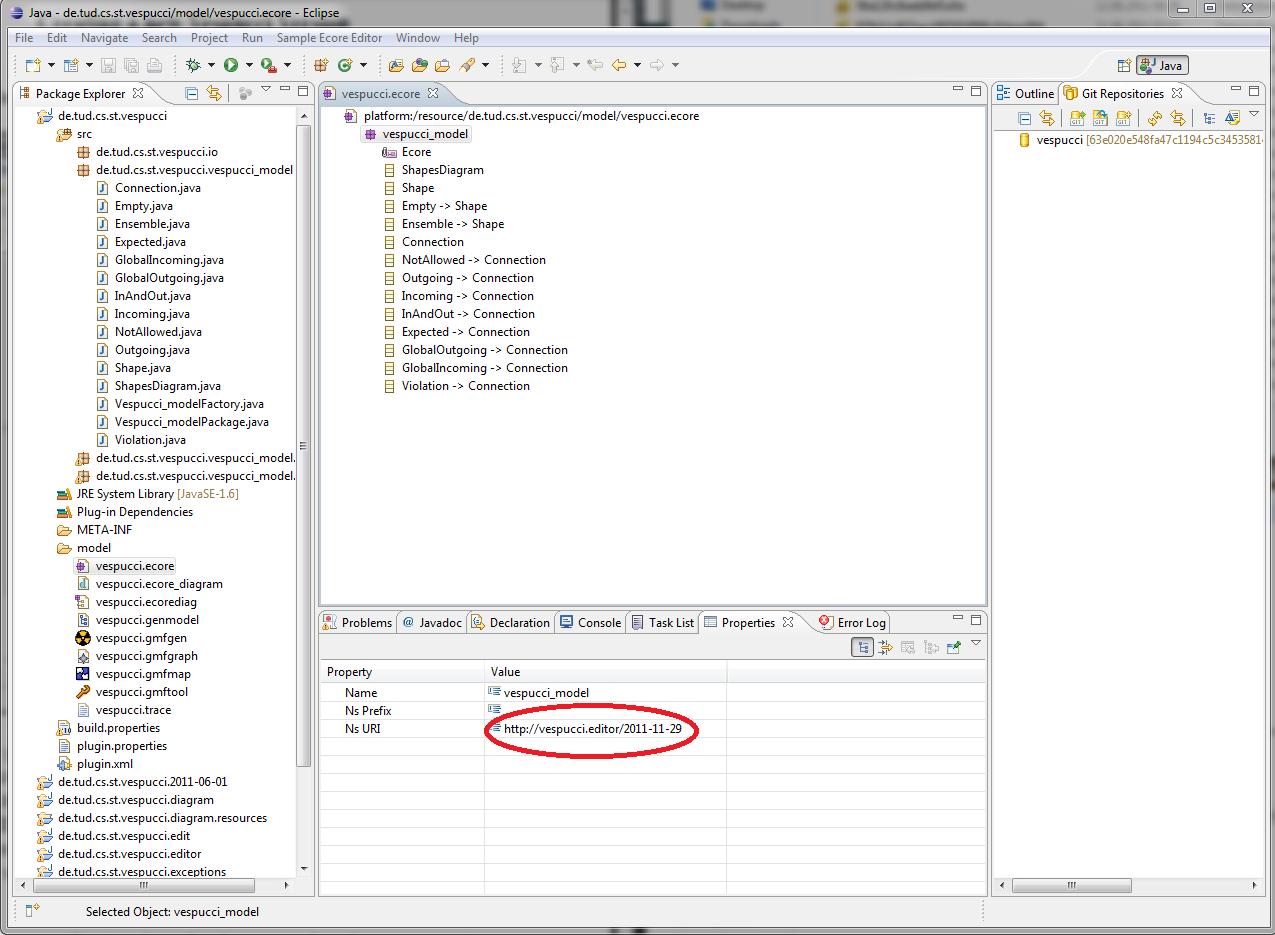
\includegraphics[width=15cm]{NsURI.png}
\\ \\After you have done that, regenerate the code and all autogenerated classes are
updated. You only have to change 'Ns URI' in the file 'vespucci.trace' manually,
which can be found in the same folder as 'vespucci.model'. If you modified plenty of the model, for example 'refactoring', you may additionally need the predecessor
version of the project in your workspace. Then you can use it in the next step by
Metamodel Mapping.

\section*{Transformation specification \footnote{written by Alexander Weitzmann and updated by Tanya Harizanova}}
The transformation specification describes how to update from one version to another. For every new version a new transformation must be specified; if that is not the case a new version is not needed at all. The transformation is realized with QVT (Query/View/Transformation). It consists of the following two parts:

\begin{itemize}
\item The \textbf{model transformation} updates the semantic model of the diagram, for example setting new relationships between semantic element or adding new ones.
\item The \textbf{notation transformation} updates the view components of the diagram, for example introducing a new (visual) description field for ensembles or changing the shape of attachments.\\ 
\end{itemize}
Existing transformations can be found in the folder 'transformation' in the 'de.tud.cs.st.vespucci.versioning' project. This is also where you should put your new QVT-transformations. Ignore the error "Cannot find operation (remember())".\\ \\
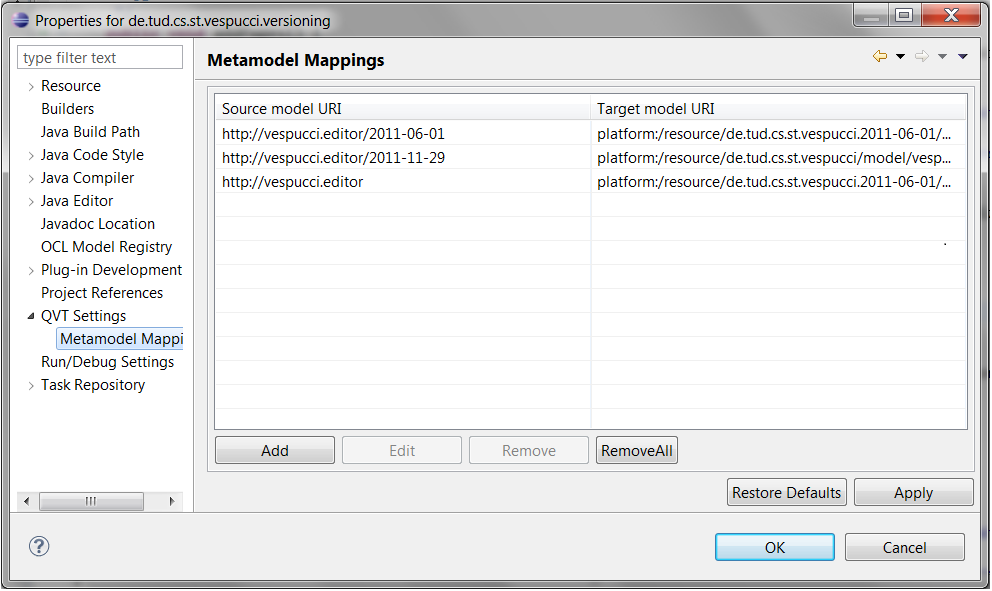
\includegraphics[width=15cm]{MetamodelMappings.png}\\ \\
\textbf{Important:} Right click on the project 'de.tud.cs.st.vespucci.versioning', then go to 'properties' $\rightarrow$ 'QVT Settings' $\rightarrow$ 'Metamodel Mapping' and add the 'Ns URI' of your Version with the path to the model of it. If you keep the old project edit its 'Ns URI' and the path to it with the right one.

\section*{Writing a new version class \footnote{written by Alexander Weitzmann and updated by Tanya Harizanova}}
New version classes are to be placed in the 'de.tud.cs.st.vespucci.versioning.versions' package. All new versions must extend the class 'VespucciVersionTemplate', which is also found in said package. This template defines all methods, which must be implemented. \\ \\ They essentially... 
\begin{itemize}
	\item point to the associated transformations
	\item point to the preceding version
	\item define the creation date, which is also the default identifier.
	\item the new namespace of the new vespucci version
\end{itemize}
\medskip
The last step is to update the field 'NEWEST\_VERSION' in the version template, that points to the newest version. You must set this to your newly created version.\\ \\
\textbf{Hint:} It is very important to add 'plugin.xml' file to your new metamodel URI and the transformations URI.\\ \\
\textbf{Hint:} Add in 'META-INF' $\rightarrow$ 'MANIFEST.MF' $\rightarrow$ 'Dependencies' $\rightarrow$ 'Imported packages' all of the project packages that are needed.

\end{document}